% Declare overall type of document (use 11pt report class on A4 paper).
% Note that the following defaults are also contained in the 'report' class
% (this is not exhaustive...see appropriate references for all options)
% 'oneside' mode...overide with 'twoside' to force output for two-sided printing.
% 'final' mode...overide with 'draft' to see linebreak malfunctioning.
% For example, to use two-sided printing one would declare the 'documentclass'
% as follows...
% '\documentclass[11pt,a4paper,twoside]{report}'
%
% Specific Mathematical options are as follows
% 'leqno' to force equation numbering on the left side of the page.
% 'fleqn' to force formulas to flush left (centered is the default).
% If 'fleqn' is specified then the left indent is controlled with '\mathindent'.
% i.e. '\setlength{\mathindent}{2.5cm}'

% Declare overall type of document (use 11pt report class on A4 paper).
\documentclass[12pt,a4paper]{turabian-thesis}

% If you want to generate an index you should include the following command
% which puts a makeindex command in the preamble. Additionally, you need to un-comment
% the file 'index' in the '\includeonly' command below and also include the 'index'
% file in the main document.
\makeindex

% Include the style file which contains all the required formatting
% information that is set out in the Research Higher Degrees Resource
% Handbook (2003 version). NOTE: This file uses the following packages
% 'graphicx' for graphics manipulation
% 'fancyhdr' for nice headers and footers.
% 'makeidx' for generating the index
% 'tocbibind' for adding table of contents entries for bibliography, index etc.
% 'sectsty' for generating stylised chapter and section headings.
% You will need to make sure your LaTeX installation has these packages
% installed...else it wont work :(
\usepackage{mathphdthesis}

% Here you would include any additional packages that you want to use.
% You should make sure they don't clash with the above packages that
% are in use in the style file.

% Specify which pieces (other .tex files) you plan to include. You can comment
% out files that you will include later or have already finished to speed
% up TeX processing
\includeonly{
prelude % Contains all the relevant candidate information (name, degrees, abstract etc)
,newcom % Place all you new commands in here
,chap1  % The first chapter
,chap2  % The second chapter
,chap3  % The third chapter
,chap4  % The fourth chapter
,app0   % Needed to switch to appendix mode
,app1   % The first appendix
,app2   % The second appendix
,biby   % Makes the bibliography from the BibTeX database
,index  % Places the index in the thesis
}

% Begin the thesis
\begin{document}

% Include all the pieces of your thesis in here.
% prelude.tex (specification of which features in `mathphdthesis.sty' you
% are using, your personal information, and your title & abstract)

% Specify features of `mathphdthesis.sty' you want to use:
\titlepgtrue% main title page (required)
\signaturepagetrue% page for declaration of originality (required)
\copyrighttrue% copyright page (required)
\abswithesistrue% abstract to be bound with thesis (optional)
\acktrue% acknowledgments page (optional)
\tablecontentstrue% table of contents page (required)
\tablespagetrue% table of contents page for tables (required only if you have tables)
\figurespagetrue% table of contents page for figures (required only if you have figures)

\title{HARMONIC BASED EXTENDED TECHNIQUES AND THEIR COMPOSITIONAL APPLICATIONS}% use all capital letters
\author{Rhys Gray}% use mixed upper & lower case
\prevdegrees{B.Mus Asc.Mus}% Used to specify your previous degrees...use mixed upper & lower case
\advisor{Matthew Boden}% example: Professor Lawrence K. Forbes
\dept{Music}% your academic department
\submitdate{November, 2019}% month & year of your thesis submission

\newcommand{\abstextwithesis}
{I propose to explore a range of extended techniques that utilise the harmonic series and assess how they can be used in my, and other people’s, creative practice. These techniques include overtones, multiphonics, and subharmonics, playable on wind and stringed instruments, and voice. While some, such as overtone singing, are well established and understood, others, such as subharmonics on stringed instruments, are still immature in terms of both repertoire and resources available.  The timbral potentials of these techniques are uncharted territories and collectively represent a whole sound world that remains relatively inaccessible to contemporary art music composers.

To ensure that only new ground is covered, I will conduct a review of the literature and resources that are readily available to composers to assess what techniques require further investigation and refinement. By researching these techniques and the mechanics behind them, interviewing industry professionals, and analysing recordings made, I hope to gain a better understanding of how the harmonic series and related techniques can be implemented in my practice. As part of both the analysis of techniques and my compositional practice, I will assess not only the compositional potential, but also the practicality of techniques. Reviewing the feasibility and notational aspects of the techniques will render the exegesis a practical document to reference when researching whether to include a technique.

I aim for my resulting exegesis to become a useful reference source for artists interested in learning about the mechanics, qualities, and potential implementations of these harmonic based extended techniques. The works that I compose accompanying the exegesis will show idiomatic treatment of the techniques and serve as references as such in the exegesis. The dissemination of the material I research will contribute to the accessibility of new sound possibilities for artists.
}

\newcommand{\acknowledgement}
{Thank you to my supervisor, Matthew Boden, my teachers Dr. Maria Grenfell and Scott McIntyre, my piano teacher Sally Ward for inspiring my passion in music, my family, and my cats Buttercup and Millie.}


% Take care of things in `mathphdthesis.sty' behind the scenes.
% Basically just does a check of all the fields that have been activated
% above and fills out the appropriate pages and adds them to the thesis.
\beforepreface
\afterpreface

% newcom.tex (new command definitions)

% Some examples (yours may be different):
\newtheorem{theorem}{Theorem}[section]
\newtheorem{lemma}[theorem]{Lemma}
\newcommand{\bfx}{{\ensuremath{\mathbf{x}}}}

% chap1.tex (Chapter 1 of the thesis)

% Set page numbering to arabic the first time we commence a chapter.
% This is required to get the page numbering correct.
\pagenumbering{arabic}

% Note that the text in the [] brackets is the one that will
% appear in the table of contents, whilst the text in the {}
% brackets will appear in the main thesis.
\chapter[INTRODUCTION]{INTRODUCTION}

\section{Methodology}
My research topic “Harmonic Based Extended Techniques and their Compositional Applications” is a review of techniques, and how they can be incorporated in my own practice. As such, it is highly subjective, and the research methodology will reflect this, being largely qualitative based. Quantitative based research, such as the analysis of techniques using spectral analysis will be used to support subjective claims. Each technique will be reviewed individually, as they are discrete from one another. Because many of the techniques are uncommon or difficult, consultation with players is paramount to undertake a fair assessment of the techniques. Document analysis of technique manuals will augment oral history research into the qualities and attributes of techniques. 
To make an educated opinion on the value of a technique, data must first be collected. Compilation of techniques both in isolated, controlled environments, and in context in musical works will allow a full and accurate use of the analytical method on recordings. Using a Fast Fourier Transformation as in Pablo E. Riera’s thesis on saxophone multiphonics, the prominent harmonics of each technique will be uncovered, for harmonic analysis.  Examination of techniques in musical context will allow for value judgements to be made about the musical effectiveness of the technique. The recorded data will be treated, and then interpreted and analysed, with the results being implemented in new works.  Through this process, my research will feed into my practice.
A holistic approach, taking both the sound possibilities and the player implications (“is this technique too difficult for the average player?”, “do I need to write for specific artists if I want to use this technique?”, etc.) is necessary to evaluate its overall potential for incorporation in my practice. To overcome this, oral history methodology will be used to gather first-hand experiences and opinions on techniques. In Bonnie Mara Barnett’s “Aspects of Vocal Multiphonics”, she conducts several interviews with singers to better understand the way the technique functions from a performer’s perspective.  Interviewing musicians able to play these techniques will deepen my understanding of the mechanics and technical aspects of creating these techniques. While my research is concerned with how I personally can incorporate these techniques into my practice, an effort to interview peer composers will be made, especially those that share common compositional traits with me. Their experiences with composing for these extended techniques will provide more data points to draw comparisons from, and contemporary composer’s compositions and feedback were a valuable component of Dr. Sarah Watts’ thesis to assess the effectiveness of the techniques. 
Augmenting the interviews, document analysis will be used on technique manuals that detail the production and quality of techniques. By building off the framework of classification articulated in Robert Dick’s seminal “The Other Flute” and extending it to accommodate a variety of techniques, comparisons across different techniques will be able to be made.  Through this, an understanding of the technical and mechanical aspects of the techniques will be gained. Techniques will be assessed on their practicality, ease of use, timbral qualities, and compatibility with my practice. Notation for the techniques varies from composer to composer, and where a common notational standard has not been developed (such as violin subharmonics), a document analysis of current notational standards will be undertaken, making reference to Elaine Gould’s seminal text on music notation, “Behind Bars”.  Through this, and subsequent consultation with players, development of a consistent and effective notational language can be achieved.
Through the collection of data from a multitude of sources and a range of different methods, it will become evident how harmonic based extended techniques are to be treated idiomatically. By undertaking a holistic review of the techniques including performer and composer points of view, the qualitative research I perform will enable not only me to incorporate these techniques into my own practice, but future composers that are interested in these techniques.

\newpage
\section{Literature Review}
This study builds on and contributes to the catalogue of resources available to composers interested in implementing harmonic based extended techniques in their practice. The topic of “Harmonic based extended techniques and their compositional applications” is broad, and I will be unable to explore the entire corpus of techniques available to all instruments. This is by design, as certain instruments lack certain facets of research, while others are already well documented, the most obvious example being string harmonics, which are common practice. This broad topic affords a certain level of flexibility to explore what is both novel and feasible given my available resources, all under the unifying theme of harmonic based extended techniques.
Many of the techniques that this study deals with are still in their comparative infancy, especially notationally. As such, engraving the works produced in the course of this study is a more subjective matter, rather than the well-established practice that it normally is. A review of the available literature makes it clear that attempts have been made to standardise contemporary music notation, but have either fallen short, or are now outdated. Kurt Stone organised an international conference on new musical notation in 1974 in Ghent, Belgium, and then produced the treatise “Music Notation in the Twentieth Century” in 1980 as a result of the conference.  This, along with Gardner Read’s 1979 “Music Notation”, served as a strong base for the standardisation of music notation, but both are mired by their age and computer based notation not being widespread. It is therefore unsurprising that both omit stringed multiphonics, subharmonics, and the many other techniques covered in my study, which largely postdate publication. Gould’s 2016 book “Behind Bars” immediately became the gold standard of engraving manuals, her decades of notational and editorial experience at Faber Music lending weight to her comprehensive treatise. But the same new techniques are omitted from Behind Bars, with Gould stating: 
‘I have been highly selective in the choice of extended instrumental and vocal techniques included in this book, but it is intended that this should give the reader the facility to create notation for other techniques not in common use.’  
Gould’s book is less prescriptive than its forerunners, and focuses more on creating a consistent style language, providing the reader with the tools of standardised and codified ‘common practice’ notation to build new extended technique notation. As such, for all notational aspects, I will be drawing upon the Gould for the philosophy of engraving, if not exact notation, which has the benefit of almost forty years of introspection against its peers. 
Gould provides the tools which Ellen Fallowfield uses to construct a notation method for string multiphonics in her PhD ‘Cello Map’, which represents an excellent framework to follow; a detailed, process-oriented review of technique informs the creation of resources which are then analysed.  Fallowfield’s analysis produced the website cellomap.com, a manual of techniques for performers to use. She states that her text maps:
‘[...] “actions that a cellist can make” onto “sounds that a cello can produce”. In other words, we have tried to reduce the cello and cellist to scales of actions and sounds, and show how cellists can influence sound (loudness, overtone content, pitch…) by their actions (bow speed, contact point, stopping position…). This standpoint is a deliberate move away from providing performers and composers with catalogues of special effects and extended techniques. Instead, we would like to provide information about how the cello works that can serve the imagination of performers and composers.’ 
This approach ‘future proofs’ the thesis by abstracting the elements into their most base form, showing all of the sounds a cello can make using all of the actions a cellist can perform. While the website is comprehensive, Fallowfield seemingly avoids making any judgement calls on the compositional applications of the techniques that she reviews, and the reader is left to draw their own conclusions on the compositional effectiveness of any given technique. Fallowfield does, however, note that a repertoire gap exists for etudes exploring multiphonics for the cello, and indeed, the entirety of the string family. As part of my practice-led research, it seems fitting to compose a piece that addresses this repertoire gap. 
Bertram Turetzky’s book, “The Contemporary Contrabass” was written to exemplify the contrabass as a serious solo and melodic instrument, which was underrepresented in the literature. He theorised: 
‘[…] concertizing was the key, which in the 1950’s was impossible mainly due to the lack of literature. I attacked this problem in two directions: 1. Locating original contrabass music from the eighteenth and nineteenth centuries, and 2. Commissioning twentieth century music.’  
His practice-led research centred on seeking to understand the techniques that contemporary composers would use in solo contrabass repertoire. He deliberately omitted including any guidance or judgements on notation, or categorisations of the difficulty of the techniques, stating that ‘[…] the time between this printing and the second edition will suffice to suggest and select the best notational concepts from a more substantial literature than we possess now.’  The second edition saw Turetzky call for more experimentation with multiphonics, stating:
‘I know of no music employing string multiphonics […] this is entirely new ground, it remains for composers and performers to build the usable technique.’ 
The specification of both composers and performers being needed to ‘build the usable technique’ is peculiar, until one re-examines the context, in which Turetzky knew of these techniques, and was attempting to rectify it through commissioning new literature. Performers and researchers such as Fallowfield are necessary to establish the technique, but without composers implementing the research carried out by them, it is impossible for a ‘usable technique’ to be built.
Thomas Howell’s 1974 book, “The Avant-Garde Flute” followed Turetzky’s contrabass technique book, as part of Turetzky’s “The New Instrumentation” series, which was published by California Press until Scarecrow Press took over in 2004.  It is relatively conservative in its content, and has many omissions. Howell’s contributions are overshadowed by Robert Dick’s “The Other Flute”, which was released the following year, and was mentioned as being an invaluable resource by John Cage in the preface to his piece “Music For”.  “The Other Flute” is a thorough, if esoteric performance technique manual, presenting each fingering and its resultant multiphonics one after the other, using a chart of descriptions to specify the qualities. It specifies the following: ‘exact pitch, ease of response, starting time, stability, dynamic range, timbre, and, if present, noise level, residual tone, and degree of modulation.’  While dry to read, it is an efficient system, and provides much more information than Howell’s fingering charts, which were presented without any accompanying context. Dick sorts the multiphonics into four classes graded by difficulty. The multiphonics are presented in order of their method of production; multiphonics derived from natural harmonics, from fingerings of chromatic pitches, and those based on microtonal segments. The scope of my research is limited to the multiphonics based on natural harmonics. From the perspective of a composer, Dick’s book provides ample resources on the qualities of each multiphonic, but generic descriptions of their characteristics; enough for a composer to assess whether any given multiphonic is worth investigating with a flautist. While the scope of my research may result in focusing exclusively on stringed instruments, Dick’s method of cataloguing different fingerings is a logical and comprehensive model to follow.
The Contemporary Violin is one of the more recent books in Turetzky’s “The New Instrumentation” series. It provides a comprehensive review of various violin techniques, but attempts to shy away from any implication of notational authority, most notable in the section on multiphonics, which seems to contradict rules codified by Gould (though to be fair, the Gould postdates Strange).  Fallowfield identified issues with the presentation format of “The Contemporary Violin” in the literature review of her thesis: 
‘The reader will find [information about col legno battuto] under the first chapter heading: ‘Bowing Technique’, the subheading ‘Col legno battuto’. Later, chapter three: ‘Percussion Techniques’ includes the subheading ‘The Bow’, in which col legno battuto is described again.’ 
Though the scope of my study is significantly smaller in scale, presentation of the findings is paramount to maintain accessibility as a resource. Given that my study focuses on harmonic based extended techniques, overlap of techniques such as multiphonics is possible, and therefore needs to avoid the structural pitfalls of Strange’s layout where information is repeated. Fallowfield’s later concern of a need for a balance between subjectivity and level of detail when describing technique and sound is also relevant to both the Strange book and doubly so to the study. These manuals merely describe the qualities of various techniques, whereas my study will be dealing with the compositional applications of the techniques; taking the extra-musical content such as blending, appropriateness for use in pitch sets, and other aspects of composition into account poses a significant threat to the usability of my study due to information overload. Marcus Weiss and Giorgio Netti discuss the reasons for limiting their study to extended techniques in the introduction to their book “The Techniques of Saxophone Playing”, stating:
‘It might indeed be conceivable to compile a multi-dimensional “Encyclopaedia of Saxophone Playing” [, however] the demands on presentation and readability would be so complex as to make such a text impractical’ 
So far, all of the literature reviewed (with the exception of the Gould and other engraving manuals) has been written either with the performer in mind, or has been written by an instrumentalist. Much of the composer-focused literature is found in the form of orchestration manuals, such as Samuel Adler’s “The Study of Orchestration” and Walter Piston’s “Orchestration”.  Attempting to cover the breadth of the art of orchestration, let alone composition, necessitates the omission of extended techniques. This is the inverse of the issue Weiss and Netti encountered, where their study required an omission of ground-level theory regarding the technical aspects of saxophone playing. Read’s “Compendium of Modern Instrumental Techniques” touches upon multiphonics, but delegates to Dick, Howell, and many of the other books from Turetzky’s “The New Instrumentation” series for notation and structure.  It becomes apparent that no matter the author, instrument, or technique, the work of packaging extended technique information for composers is left to somebody else; composers seek to cover the entirety of the craft, while performers seek to cover the entirety of the instrument. Therefore, there is a dearth of resources for composers seeking to incorporate harmonic based extended techniques into their practice. My study addresses this by covering the playability, notation, and implementation of harmonic based extended techniques across relevant instruments. Through practice-based research, the exegesis produced by my study will document the process of composing using these techniques, refining the methodology and notation through the creation of several new works. The resulting document will fill a hole in literature aimed at composers by acting as a practical manual for those interested in implementing harmonic based extended techniques in their own practice.


\newpage
\section{New Section}
Here we have started a new page to show how the headers work. The
text in the header should be the last section title declared at
the end of the current page.

This new paragraph shows how to set \index{index items}index items
and \index{index items!subindex items} subindex items.

\subsection{New Subsection}
Here's a subsection with some simple maths $a^2+b^2=c^2$.

\subsubsection{subsubsection}
Here's a \index{subsubsection}subsubsection...oooooooohh....wow
wee!!!!!!

\newpage
Some more text to check indent and show how references work
\cite{Williamson:STS}.

Here's how we place a figure (Figure \ref{fig:utas}) on the page.
\begin{figure}[hbtp]
\begin{center}
\scalebox{.30}{
\includegraphics{Utas_vert_BW}} \caption{
\label{fig:utas} The UTas logo}
\end{center}
\end{figure}

And finally, here's a table example (Table \ref{tab:taba}).
\begin{table}[hbtp]
\begin{center}
\begin{tabular}{|r|r|r|r|r|}
\hline
$n=$&2&3&4&5\\
\hline
$c$ (rad/day)&1.67&0.52&0.06&-0.17\\
\hline
period (days)&3.75&12.00&100.00&37.50\\
\hline
\end{tabular}
\end{center}
\caption{\label{tab:taba}A simple table}
\end{table}

% chap2.tex (Chapter 2 of the thesis)

\chapter[THE NEXT CHAPTER]{The Next Chapter}

\section{New Section}
Here's yet another \index{section}section with an appropriate
index entry.

% chap3.tex (Chapter 3 of the thesis)

\chapter[ANOTHER CHAPTER]{Another Chapter}

\section{New Section}
More stuff here too.
% chap4.tex (Chapter 4 of the thesis)

\chapter[CONCLUSION]{Conclusion} \label{concl}

\section{New Section}
This better be good if you don't want a Masters!

% app0.tex (file to switch to appendix mode)
% No need to alter this file...
\appendix
\appendixpage
\addappheadtotoc
\newcommand{\HRule}[1]{\rule{\linewidth}{#1}}
\newcommand\invisiblechapter[1]{%
  \refstepcounter{chapter}%
  \addcontentsline{toc}{chapter}{\protect\numberline{\thechapter}#1}%
  \chaptermark{#1}}

% app1.tex (file to switch to appendix mode)


\invisiblechapter{\violinPiece}

\vspace{3.8cm}

\begin{center}

\textsc{for solo violin}

\vspace{2.8cm}

\HRule{0.5pt}

\LARGE \textbf{\uppercase{\violinPiece}}

\HRule{2pt}

\vspace{1.8cm}

\normalsize \today

\vspace{3.8cm}

Rhys Gray

\end{center}
\newpage
\section*{Program Notes}
\violinPiece is a solo work for violin that explores half-harmonics.
It is a non-programmatic work, and the title was inspired by a question that my supervisor posed to me while I sought ethics approval for my exegesis; a simple phrase laden with possible contexts, spurring the imagination to try and complete the meaning.

It is, in a way, an etude that explores half-harmonics, similar to those found in Sciarrino's \emph{6 Caprricio for violin}. 
Half-harmonics are produced by applying left hand finger pressure halfway between that required to create a harmonic, and a \emph{normale} sound. 
The sound that is produced should be a mixture of the stopped string pitch, the harmonic pitch, and a resistant, slightly noisy quality.

\section*{Notation}
\begin{itemize}

    \item Half-harmonics are notated in the score as a half-filled diamond notehead.
    \item sp denotes \emph{sul ponticello}.
    \item msp denotes \emph{molto sul ponticello}.
    \item similarly, st denotes \emph{sul tasto}, and mst denotes \emph{molto sul tasto}
\end{itemize}

\newpage

% 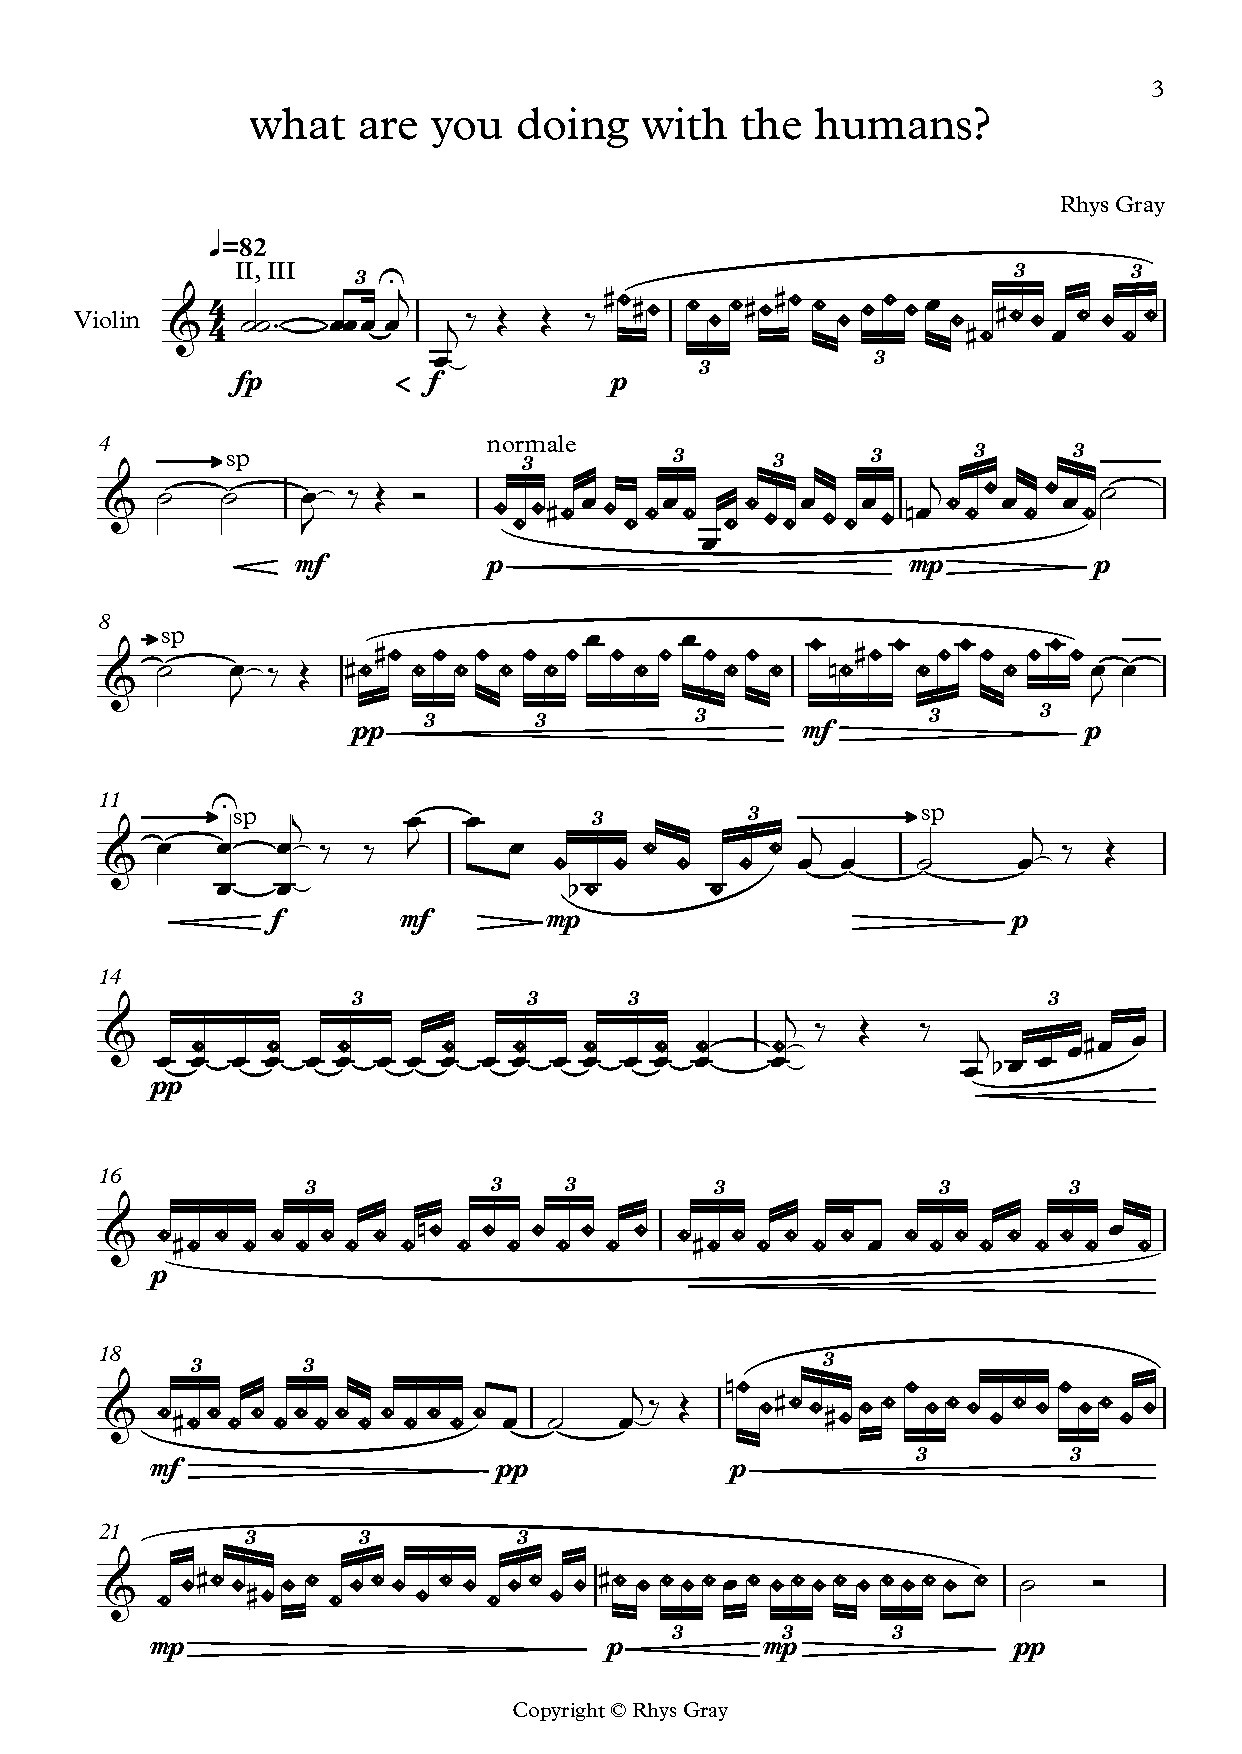
\includepdf[pages=-,pagecommand={},width=\textwidth]{resources/compositions/violin.pdf}

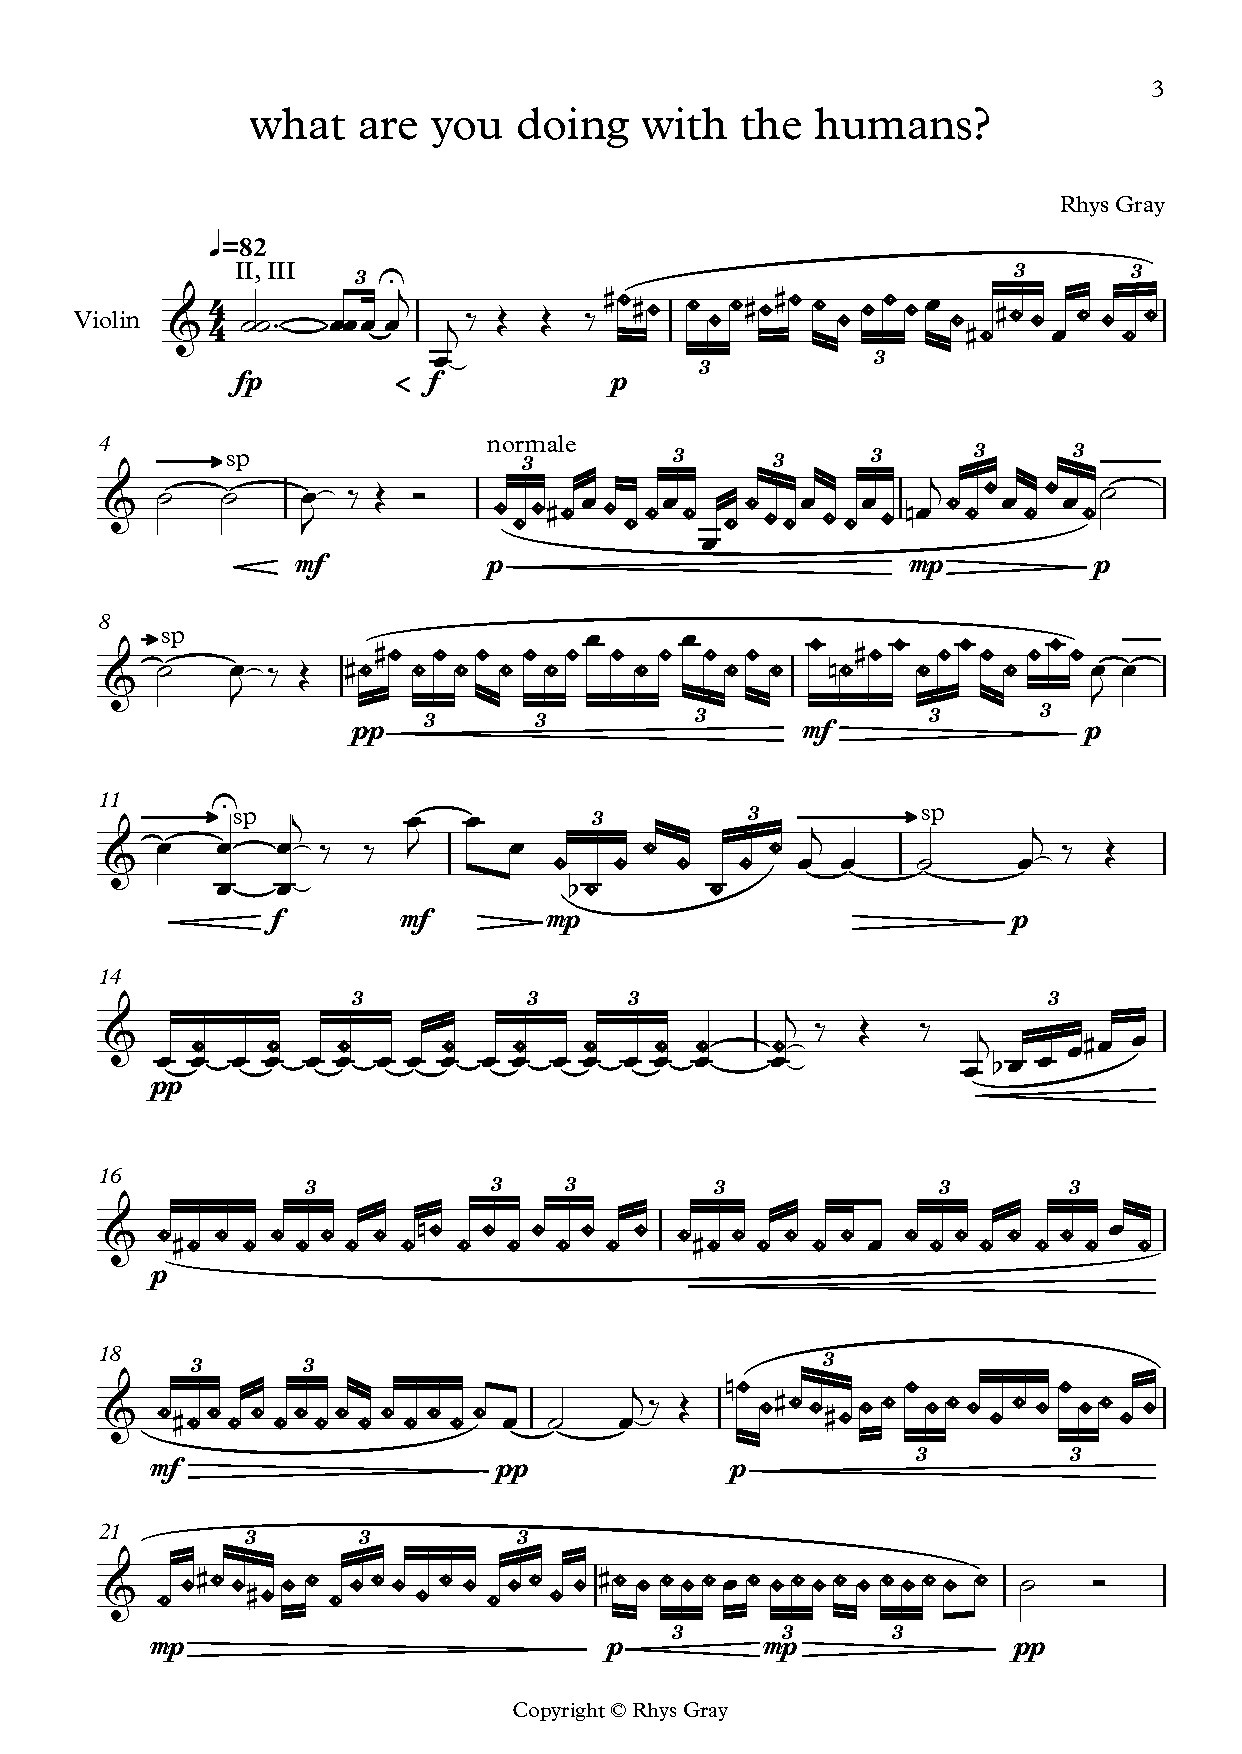
\includepdf[pages=-,pagecommand={}]{resources/compositions/violin.pdf}
% app2.tex (file to switch to appendix mode)

\invisiblechapter{\violaPiece}

\vspace*{3cm}
\begin{center}
\textsc{for solo viola}

\vspace*{3.5cm}

\HRule{0.5pt}


\LARGE \textbf{\uppercase{\violaPiece}}
\HRule{2pt}

\vspace{1.3cm}

\normalsize October, 2019
\date{}

\vspace*{5\baselineskip}

Rhys Gray

\end{center}
\newpage
\newpage

\section*{Program Notes}
\emph{Doppelganger} is a piece for solo viola, written to explore the lower register of the viola using \hyperref[sec:subharmonics]{subharmonics} juxtaposed with upper harmonics. 

To play subharmonics, one should place the bow at the 6th partial of the harmonic series of the fingered pitch, and bow with excessive pressure and an absolutely consistent speed. 
The increased pressure will distort the vibration of the string, producing a phase loop which, in turn, produces the subharmonic. 

Subharmonics are achieved through precise control of torsional oscillation, which usually produces the sound of an amateur string player's heavy handed, slow bowing. 

The production of subharmonics can be aided by using older strings (which work better due to fats building up on the strings). 
Making a counter-clockwise half-twist in the string can also make it easier to produce octave and major second subharmonics (additional twists can help achieve lower subharmonics, at the expense of higher ones).

\section*{Notation}
\begin{itemize}

    \item Subharmonics are notated in the score using a square notehead for the fingering, with a small notehead at the desired resultant pitch.
    \item sp denotes \emph{sul ponticello}.
    \item msp denotes \emph{molto sul ponticello}.
    \item similarly, st denotes \emph{sul tasto}, and mst denotes \emph{molto sul tasto}
\end{itemize}

\newpage\label{app:doppelganger Score}

% 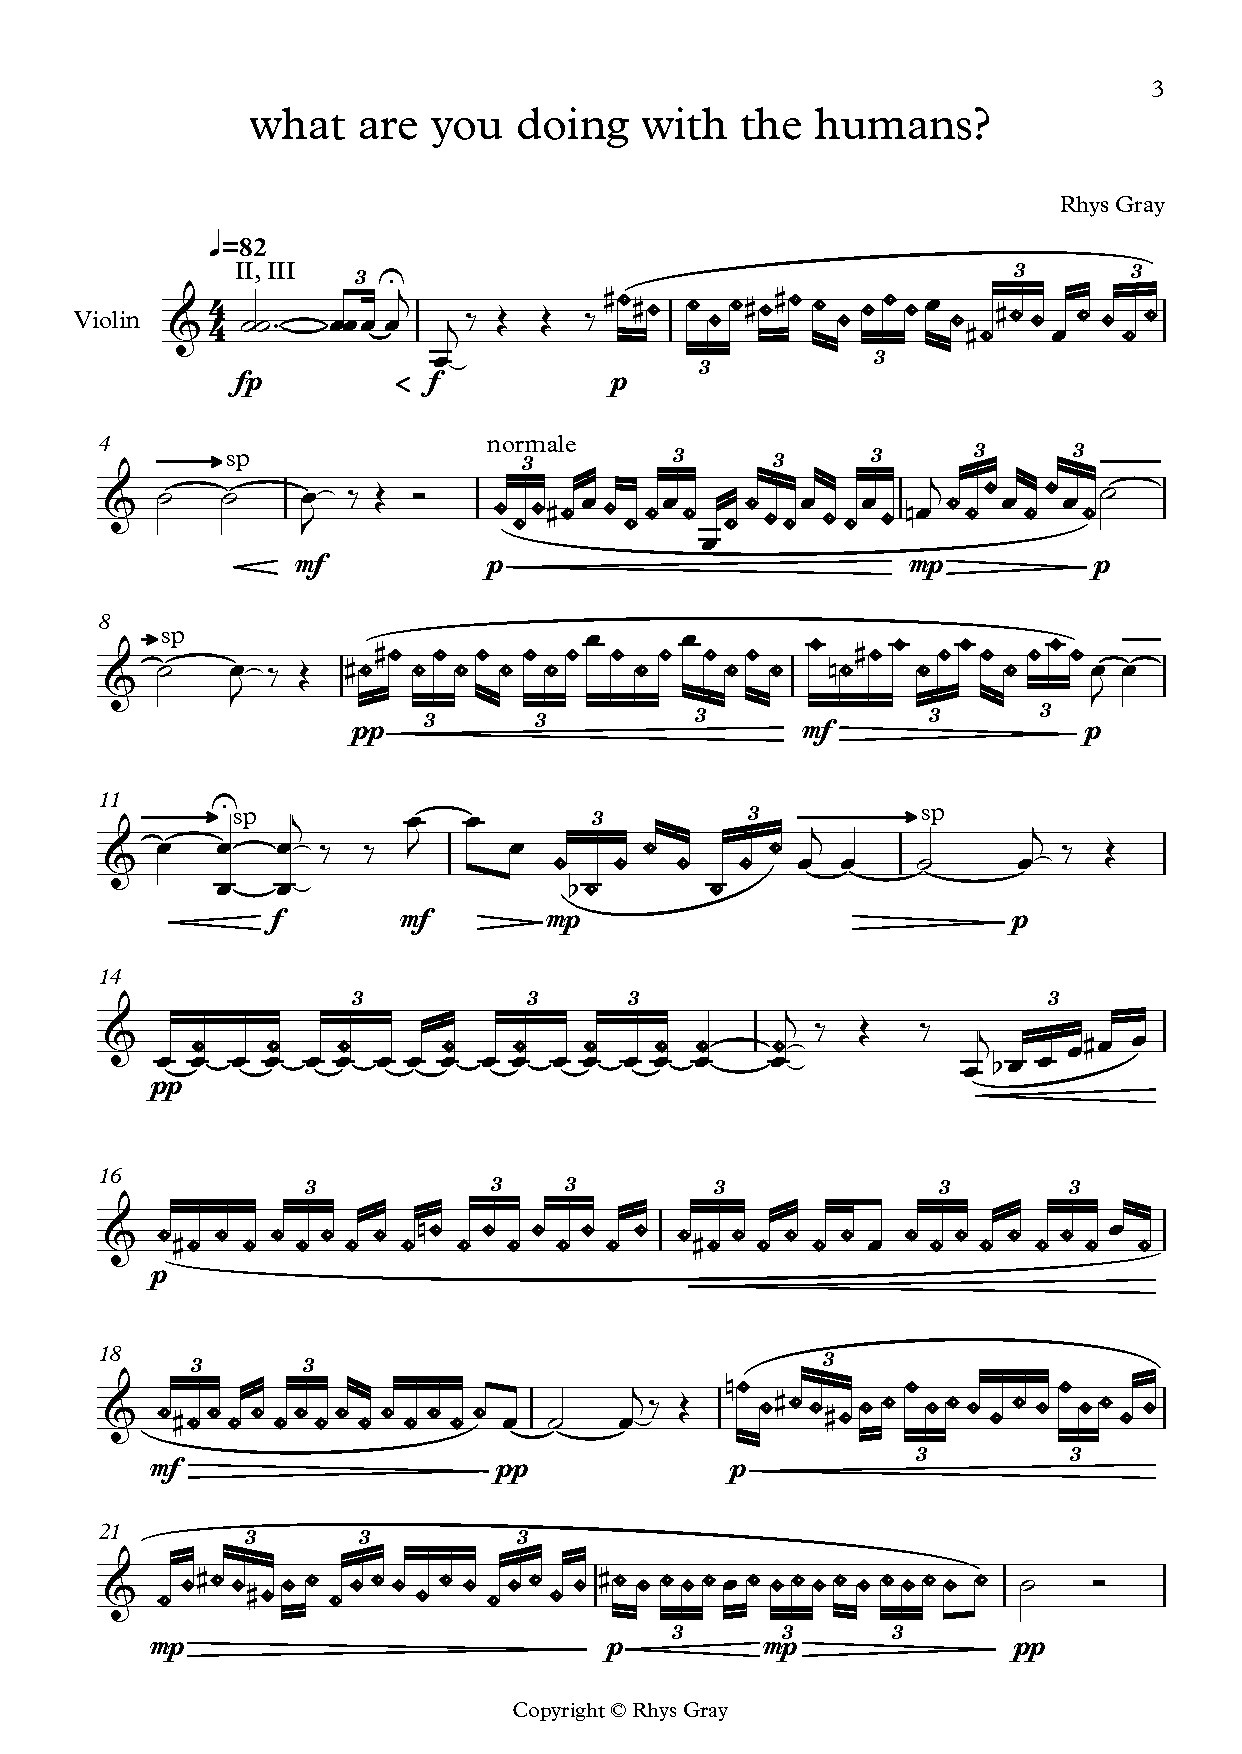
\includepdf[pages=-,pagecommand={},width=\textwidth]{resources/compositions/violin.pdf}
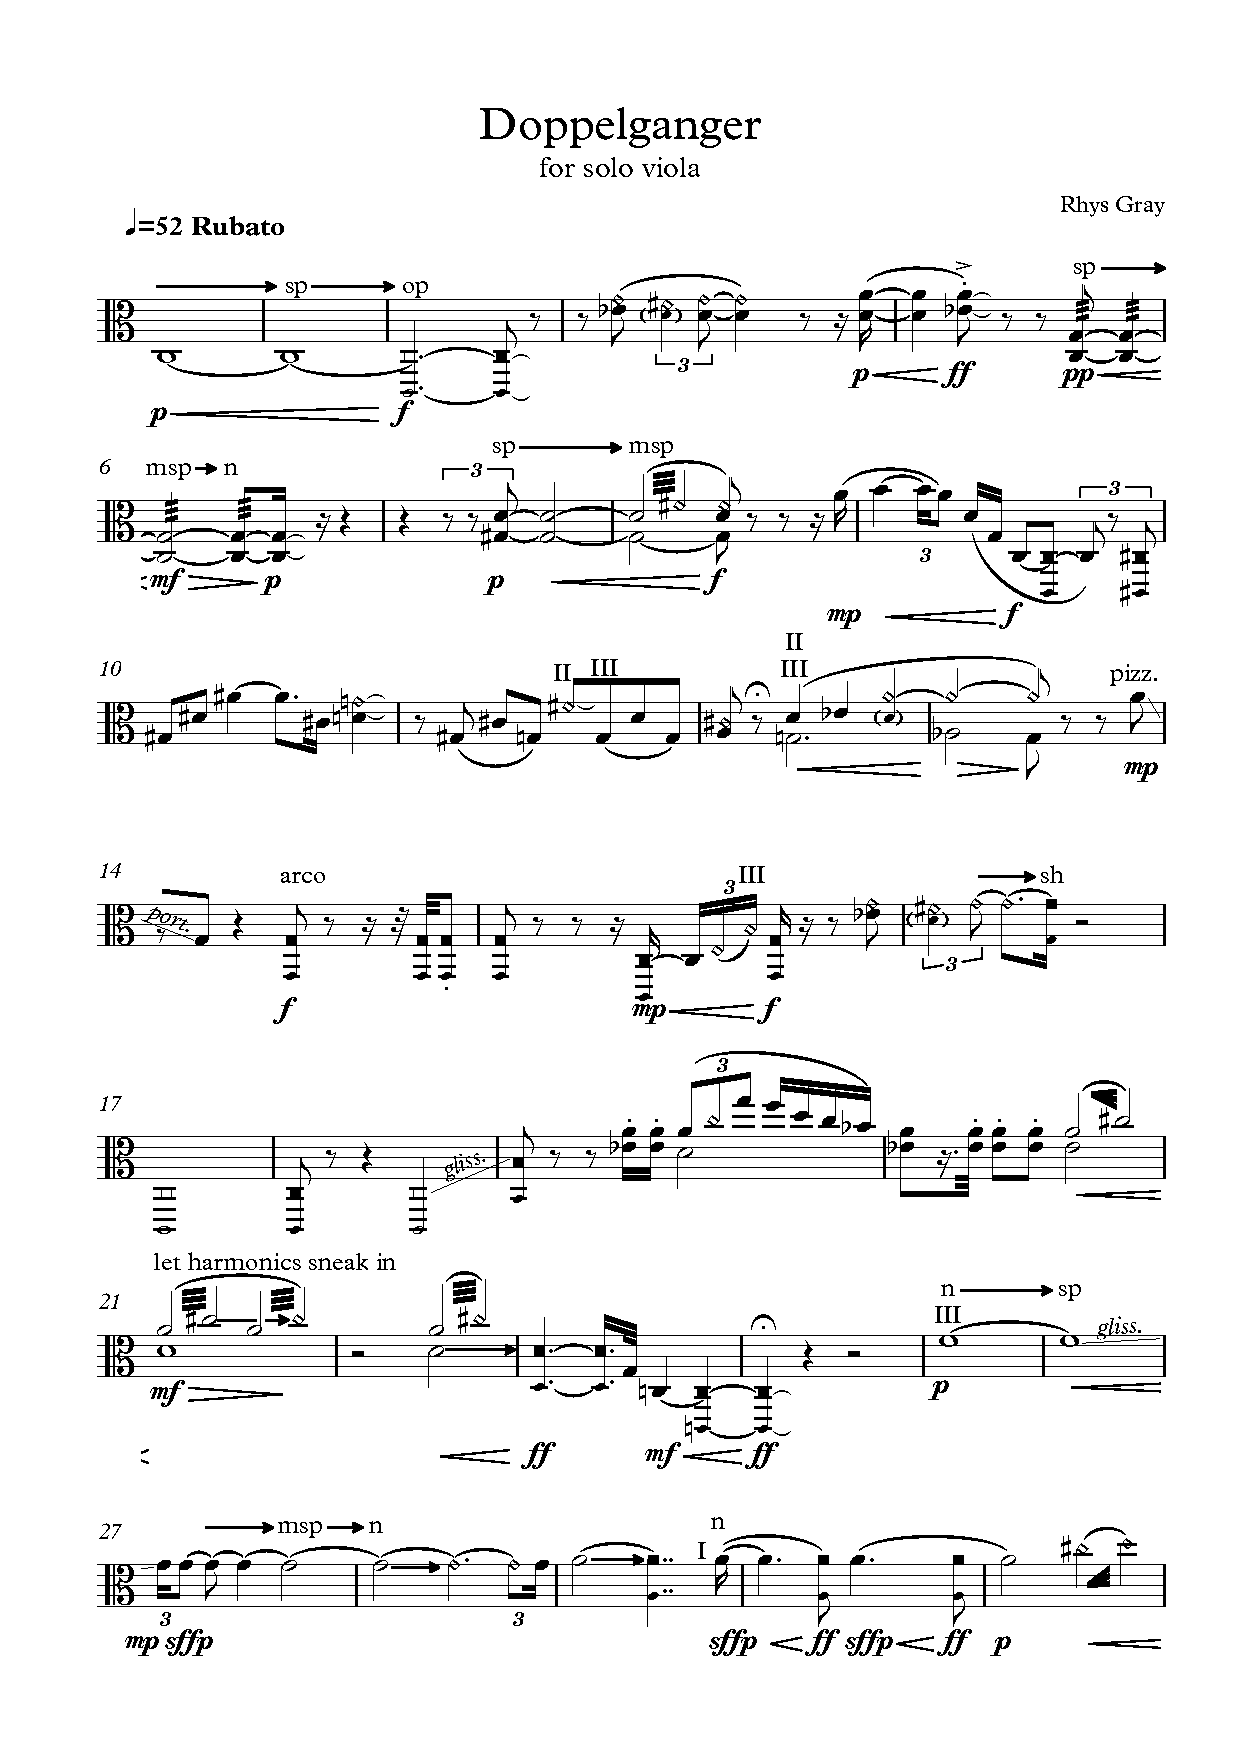
\includepdf[pages=-,pagecommand={}]{resources/compositions/viola.pdf}
% Add in the bibliography
% Set the text size to be small
\small
% Set the bibliography style to be plain.
\bibliographystyle{plain}
% List all citations in thesis.bib file
% Comment this out for final printing
% if you have un-cited items in your
% bib database
\nocite{*}
% thesis.bib is the name of our database
% and we load it with the following command
\bibliography{thesis}

% A small file that prints the index in the main document.
% No need to alter this file...
\printindex


\end{document}
